\documentclass{article}
\title{TDA297 Laboration 2}
\author{anordin@student.chalmers.se\quad Anders Nordin\\
        viklin@student.chalmers.se\quad Viktor Lindstr\"{o}m}
\date{\today}
\usepackage[T1]{fontenc}
\usepackage[utf8]{inputenc}
\usepackage[english]{babel}
\usepackage{verbatim}
\usepackage{enumerate}
\usepackage{steinmetz}%för att få tillgång till /phase
\usepackage{amsmath}%massa trevliga symboler
\usepackage{siunitx}%enklare notation på enheter
\usepackage{tikz}
\usetikzlibrary{arrows,decorations.pathmorphing,backgrounds,positioning,fit,petri}
\usepackage{fullpage}
\begin{document}
\maketitle
\newpage

\section{Introduction}
  This report describes a protocol on how to maintain total order 
  as well as causal order in a system that has reliable unicast FIFO order messaging.\\
  In this protocol a single node is elected as a sequencer and all messages is sent through
  the sequencer and it will then singlehandedly add sequence numbers and then broadcast it
  to all other nodes.
  The report will start with a short description of the system and what algorithms used. 
  Then reliability is discussed and how the system solve integrity, validity and agreement.
  After that an explanation of how the system holds for total and causal order. Then there 
  is an explanation of how the system handle crashing processes. Lastly there is a conclusion.

\section{Description of the system}
 The system consists of N processes that communicate with each other by TCP channels.
 TCP channels gives the system reliable unicast with FIFO order. Upon this system a
 reliable total and causal order broadcast is implemented. 
 In order to handle crashing nodes, flooding is used. When a process receive a message
 it is then sent to the other processes. 
 In order to handle order a single process called sequencer is used which handle all
 ordering of messages.
 \subsection{Sequencer}
 \label{sequencer}
 In this system there exists a single node that is also a sequencer. All messages will 
 pass through the sequencer and the sequencer will then add a sequence number to that 
 message, and then distribute it to all nodes. The nodes will then receive the message 
 and then start flooding it to all other nodes. These events is described by Figure 
 \ref{fig1}. An important thing to note in the figure is that the sequencer is described 
 as an independent node. This is for simplification, in reality the sequencer is kept 
 within a node. \\
 \subsection{Nodes}
 The normal nodes will send its message to the sequencer, get it back with a sequence number.
 In order to then create the correct order, the messages is not delivered directly when
 it is received, but is instead put in a queue until the correct sequence number is acquired.\\
 \subsection{Example}
 Example of two functioning nodes with a sequencer. The message sent to the sequencer is 
 represented by a wavy arrow, and the messages with a sequence number is represented by normal
 arrows.
  \begin{figure}[h]
    \centering
    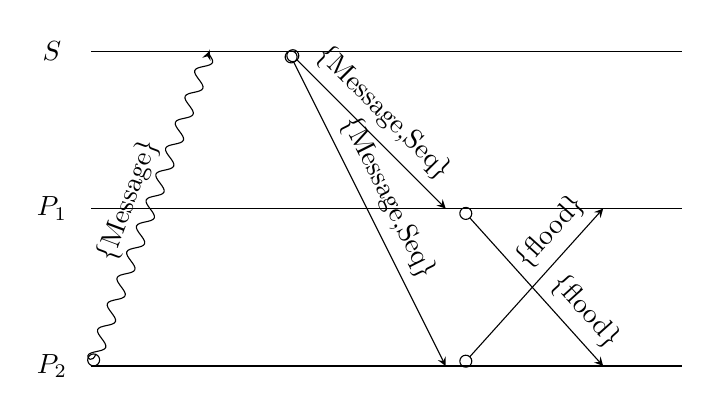
\begin{tikzpicture}
      \draw (0,0) node{$P_2$} (0.5,0) -- (8,0);
      \draw (0,2) node{$P_1$} (0.5,2) -- (8,2);
      \draw (0,4) node{$S$}   (0.5,4) -- (8,4);

      \draw [decorate, decoration=snake, o-stealth,anchor=south,sloped] (0.5,0) -- 
          node {\{Message\}}    (2,4);
      \draw (3,4)[o-stealth,anchor=south,sloped] -- 
          node {\{Message,Seq\}} (5,2);
      \draw (3,4)[o-stealth,anchor=south,sloped] -- 
          node {\{Message,Seq\}} (5,0);

      \draw (5.2,0)[o-stealth,anchor=south west,sloped] -- 
          node {\{flood\}} (7,2);
      \draw (5.2,2)[o-stealth,anchor=south west,sloped] -- 
          node {\{flood\}} (7,0);
    \end{tikzpicture}
    \caption{Example of a message being broadcasted}
    \label{fig1}
  \end{figure}
  
  \subsection{Assumptions}
  The system is built upon the following assumptions:
  \label{assumption}
  \begin{itemize}
  \item Reliable unicast
  \item FIFO-order unicast
  \item No partitioning in the network
  \end{itemize}  

\section{Reliability} 
  \label{reliability}
  %Short description here, proofs in subsections!
  The reliability is provided by flooding the message. By the assumptions made in \ref{assumption} we can rely on 
  that each single message sent by a working process $P_i$ to its neighbours $P_j$ to $P_n$ will be delivered.
  And hence the sequencer is the only one that sets the sequence number the number is preserved within the message.
  
\subsection{Integrity}
As the messages arrive at the process it is stored in a buffer implemented as a set. With the help of sequence numbers
it is possible to assure that the message is only beeing delivered once. The process only delivers the message if it
has not already been delivered. Therefore no duplicates exists in this solution. If a process dies another node will flood
the message to the rest working processes.
% What will happen when a process crash?
% We use seq nr to assure the we dont have any duplicates. Stored in set(no duplicates).
% "Each process delivers a message at most once from another process. The message must been broadcasted earlier"


\subsection{Validity}
As described earlier in the section \ref{sequencer}, all messages that are broadcasted is first sent to the sequencer which
later broadcasts the message to all processes. This part can assure that the message is broadcasted atomically, either the complete
message is sent or it is not sent at all. If a leader dies during broadcast at least one process will eventually get the message and 
may in turn flood the message to the rest processes which will in turn flood the message. What is meant to say is that all processes
share the same set of messages. This applies for any node.

% The set beeing delivered must contain all  msgs that have been broadcasted by correct processes"
% Flooding is the key and like we said no netwrok partions. 
% Atomic broadcast, once one peer has the msg everyone will get it by flooding principle.

\subsection{Agreement}
Since the property of validity already applies for this solution it is safe to say that if a $P_n$ have the set delivered with all
messages that have been broadcasted by a correct process, a process $P_(n+1)$ also has that.
% All correct processes will eventually deliver same set of msgs"
% Same as validity, if it applies for one it applies for all.

\section{Ordering}
  It is important in the protocol that the order of the messages is the same 
  for all members of the network. Therefore in the following subsection it is 
  described how the protocol satisfy total and causal order.

\subsection{Total order}
  The sequencer is the only one that takes care of the ordering. 
  No one else is allowed to set a sequence numbers. If a message 
  is sent, it has to be passed to the sequencer, get a sequence 
  number, and then it is delivered back by a broadcast. When it 
  is received it is not delivered, it has to be put to a queue 
  untill the message with the next sequence number if found. 
  Hence there is only one node that is allowed to set sequence 
  numbers, and the  sequence numbers is unique, all the nodes 
  will get a message with a sequence number.
  
\subsection{Causal order}
  %Each message has to be sent by one single process S in the group g.
  Assume towards contradiction there can exist a message sequence
  that breaks causal order, then a process $P$ has to received a message $m_1$
  after that send a message $m_2$, this causes $m_1$ and $m_2$ to be causally
  related. To break the causal order, message $m_2$ has to be percieved before $m_1$, 
  but this is a contradiction hence message $m_1$ has to have a sequence number when 
  it is received by $P$ and $m_2$ will get a higher sequence number when it is sent 
  to the sequencer, and the nodes deliver the messages according to the sequence numbers.
\section{Fault tolerance}
  Fault tolerance in failing nodes is already described in section \ref{reliability}.
  An important notice that is not to be forgotten is the sequencer. If the sequencer 
  dies, a new sequencer has to be elected and integrity, validity and agreement will 
  still be preserved aswell as ordering.
  \subsection{Integrity}
    When a node is sending a message, one and only one, is created and then put in a queue.
    the message together with an unique id specific for that processor. When the message then is 
    received from the broadcast it is then removed. This means that if and only if a message is 
    sent, it    will be present in the sending nodes send buffer, and if and only if the message
    is broadcasted it is removed from the buffer. No where will it be duplicates.
    
  \subsection{Validity}
    If a node containing the sequencer crashes, the other nodes will place their messages in their
    send buffer and then try to send them, when they realize that the node is unreachable, a new 
    sequencer is elected. The elected node will then send a message to the other nodes updating them
    about a new sequencer is elected, and it is to this nodes the following messages should be sent.
    The nodes will then send the messages it was unable to send to the previous sequencer to the
    new sequencer, and they will then be broadcasted and removed from the buffer to inform the nodes
    that the message is infact broadcasted.

  \subsection{Agreement}
    When a new sequencer is elected, the elected process will send a special message to the other nodes
    that it is the new sequencer, hence the single one is elected, and it and only itself sends the 
    messages to all other nodes to be updated, no one will be without a notion of the new leader

  \subsection{Ordering}
    If the sequencer dies, then the nodes will buffer their messages untill it is received. 
    All theise messages will then be concurrent if the sequencer is dead, hence no one can 
    deliver a message untill a new sequencer is elected, and no need for flooding or special
    ordering is needed. When the new sequencer is found the nodes just have to send their messages as soon
    as possible, but before anything else, to the sequencer. Hence causal order will be preserved, no one
    can recieve messages while the sequencer is dead and they will be causally concurrent. The new sequencer
    will set sequencer numbers and broadcast the message exactly as before so total order is also preserved
    hence it is buffered in each node and then delivered according to sequence numbers.
    
\section{Conclusion}
  The solution might seem crude at a beginning, but the fact is that the message complexity
  is rather good in this solution.To broadcast a message, one message is sent to the sequencer and then N 
  messages is sent to each node, where N is the number of nodes in the group, as opposed to a aproach
  where each node has to agree on a sequence before the message is sent. This generates order of N messages
  even before the message is sent, then the message has to be broadcasted, making the message complexity
  being atleast double. Although, one have to keep in mind that our solution sends a whole message
  to the sequencer, and the agreement aproach just has to agree on sequence, which can be done with
  small messages. The bad thing is that it sends alot of data through the sequencer and the node 
  that acts as a sequencer might be overloaded with messages, and if it dies no one will be able 
  to send any messages untill the new one is elected.
\end{document}
